\documentclass[12pt]{article}

\usepackage{listings}
\usepackage{color}
\usepackage[utf8]{inputenc}
\usepackage{float}
\usepackage{amssymb}
\usepackage{amsmath}
\usepackage{graphicx}
\graphicspath{ {./images/} }

\DeclareFixedFont{\ttb}{T1}{txtt}{bx}{n}{12} % for bold
\DeclareFixedFont{\ttm}{T1}{txtt}{m}{n}{12}  % for normal

% Custom colors

\definecolor{deepblue}{rgb}{0,0,0.5}
\definecolor{deepred}{rgb}{0.6,0,0}
\definecolor{deepgreen}{rgb}{0,0.5,0}


% Python style for highlighting
\newcommand\pythonstyle{\lstset{
language=Python,
basicstyle=\ttm,
morekeywords={self},              % Add keywords here
keywordstyle=\ttb\color{deepblue},
emph={MyClass,__init__},          % Custom highlighting
emphstyle=\ttb\color{deepred},    % Custom highlighting style
stringstyle=\color{deepgreen},
frame=tb,                         % Any extra options here
showstringspaces=false
}}


% Python environment
\lstnewenvironment{python}[1][]
{
\pythonstyle
\lstset{#1}
}
{}

% Python for external files
\newcommand\pythonexternal[2][]{{
\pythonstyle
\lstinputlisting[#1]{#2}}}

% Python for inline
\newcommand\pythoninline[1]{{\pythonstyle\lstinline!#1!}}

\author{Simone Jovon 882028}
\title{Assignment 2: Discriminative and Generative Classifiers}

\begin{document}
\maketitle

\section{Task Description}

The goal of the assignment is to write a handwritten digit classifier for the 
\textbf{MNIST database}\footnote{\textit{http://yann.lecun.com/exdb/mnist/}}. 
These are composed of 70000 28x28 pixel gray-scale images 
of handwritten digits divided into 60000 training set and 10000 test set.

We have to train the following classifiers on the dataset:
\begin{enumerate}
    \item SVM  using \textbf{linear}, \textbf{polynomial of degree 2}, 
            and \textbf{RBF} kernels;
    \item Random forests;
    \item Naive Bayes classifier where each pixel is distributed according to a Beta 
          distribution of parameters $\alpha$, $\beta$:
          $$
          d(x,\alpha,\beta)=\frac{\Gamma(\alpha+\beta)}{\Gamma(\alpha)\Gamma(\beta)} x^{(\alpha-1)} (1-x)^{(\beta-1)}
          $$
    \item k-NN.
\end{enumerate}

For SVM and random forests we can use any library we want, but we must implement 
the Naive Bayes and k-NN classifiers.

\section{Theoretical Background}

Let's start by defining what is \textbf{supervised learning}: given a set of example
input and output  pairs find a function that that does a good job of predicting the
output associated to a new input. 
Having said that, all classifiers that we will see in this report are supervised 
learning models.

A classifier needs to be trained on a dataset to be able to predict, in the best
possible way, the output of new data (classification). 
On large datasets the data is split in two parts:
\begin{itemize}
    \item \textbf{Tainig set}, to train the classifier;
    \item \textbf{Test set}, to test how accurate are the predictions of the classifier
            over new data.
\end{itemize}

During the training process the classifier don't have to fit the training date 
too precisely, because this can lead to bad results on new data, this problem is konwn
as \textbf{overfitting}. 

\subsection{Support vector machine (SVM)}

If a dataset can be split by a linear separator the data space is called
\textbf{linear separable}, when we faced a non-linearly-separable dataset we can take
two approaches:
\begin{enumerate}
    \item use a more complex separator;
    \item use a linear saparator and accept some errors.
\end{enumerate}

Support vector machine performs a linear classification, but with a trick called 
\textbf{kernel trick} it can also performs non-linear classification.

In general, there can be multiple separators for a dataset, a natural choise, and
the one adopted by SVM, is to choose the one with the largest geometric margin.

In the case of a "nearly" separable dataset we may be willing to have a separator
that allows a small misclassification by making the margin condition less strict.
So it can be introduced a variable C that controll how much strictly the margin 
must be enforced, choosing a big value of C the classifier will work very hard
to correctly classify
all the data set, a lower value of C instead allows more easily a 
misclassification of the point to achive a better margin.

On non-linearly-separable dataset if we transform the feature values of the points
inside the dataset in a non-linear way, we can trandform the dataset into one that
is linearly separable. To adapt the dataset to the new feature space a function 
$\phi(x)$ is used, the $\phi$ function can map the values of the dataset also to 
an higher-dimentional space and it can do a non-linear transformation.

Since SVM only use a dot product of the data
\begin{itemize}
    \item $\phi(x_i) \cdot \phi(x_j)$, to train the classifier
    \item $\phi(x_i) \cdot \phi(u)$, to classify a new point
\end{itemize}
there is no need to compute $\phi(x)$ to every single point x, but having
$$
    \phi(x_i) \cdot \phi(x_j)  = K(x_i, x_j)
$$
we can simply define the function 
$K : X \times X \to\mathbb{R}, \{x_1,\dots x_n\} \subseteq X$, such function is 
called \textbf{kernel}.

There are various choises for kernels:
\begin{itemize}
    \item \textbf{Linear kernel}: $K(x_i, x_j) = x_i \cdot x_j$
    \item \textbf{Polynomial kernel}: $K(x_i, x_j) = (1 + x_i \cdot x_j)^n$
    \item \textbf{Radial Basis Function}: $exp(- \frac{1}{2} \frac{\|x_i-x_j\|}{\sigma^2})$
\end{itemize}

\subsection{Random forests}

Decision trees can be seen as rules to perform categorization, but how to create a
good decision tree that makes corrects categorization of new data? The main
problem is to decide which node put in which position. This problem can be easily
solved using an alghorithm like the ID3 Alghorithm, that using a measure 
called \textbf{Information Gain} it decides which node to put next on the tree.

Decision trees after the training can perfectly fit the given dataset but may
not be so accurate to classify new data, so there may be overfitting.
The Random forests solves this problem by constructing a multitude of 
decision tree during the training.

Before going further let's introduce a training technique called 
Bootstrap Aggregating (\textbf{Bagging}); given a training set it 
selects some random samples with replacement of the training set and it creates the 
associated decision trees. Having this set of decision trees, the predictions of the 
classifier is the average of the predictions of the various decision trees.

The training alghorithm for random forests follows the 
Bagging procedure but with a small difference; each time a split is to be performed, only a random subset of features is
selected to create the associated decision tree. 

\subsection{Naive Bayes classifier}

The Naive Bayes classifier have a \textbf{generative} approach instead of a 
\textbf{discriminative} one,
so this classifier given a training set tries to create models that represents the
various classes.
 
To classify a new data we match the date with all the models, then see which model 
represents better the new data.

In more formal therms, \textbf{discriminative} algorithms try to learn $p(y|x)$, 
instead \textbf{generative} algorithms try to model $p(x|y)$ and $p(y)$.

With a Naive Bayes classifier, to classify a new data $x = \{x_1,\dots x_n\}$ we have 
to compute for every class $c$
$$
p(x, y=c)=p(x \mid y=c) p(y=c)=\left(\prod_{i=1}^{n} p\left(x_i \mid y=c\right)\right) p(y=c)
$$
and choose the model that have the higher joint probability.

On our classifier each pixel is distributed according to a Beta distribution of 
parameters $\alpha$, $\beta$
$$
p(x ; \alpha, \beta)=\frac{\Gamma(\alpha+\beta)}{\Gamma(\alpha) \Gamma(\beta)} x^{\alpha-1}(1-x)^{\beta-1}
$$
with
$$
\begin{aligned}
& \alpha=K E[X] \\
& \beta=K(1-E[X]) \\
& K=\frac{E[X](1-E[X])}{\operatorname{Var}(X)}-1
\end{aligned}
$$

\subsection{k-nearest neighbors (k-NN)}

Let's start by defining $P$ as the probability that a vector fall into a region $\mathcal{R}$
$$
    P=\int_{\mathcal{R}} p(x) d x
$$
if we assume that $\mathcal{R}$ is small enough that $p(x)$ doesn't vary so much inside it,
we can redefine $P$ as
$$
    P=\int_{\mathcal{R}} p(x) d x \approx p(x) \int_{\mathcal{R}} d x=p(x)|\mathcal{R}|
$$
After a Monte Carlo estimation of the probability $P = \frac{k}{n}$ as the proportion
of vectors ($k$) of the sample ($n$) fall within $\mathcal{R}$ we have that
$$
    p(x) = \frac{k/n}{|\mathcal{R}|}
$$
Now assume k to be constant and enlarge the window until we find enough samples, if
we let the number of neighbors $k(n)$  grows to infinity more slowly than n
$$
    \lim _{n \rightarrow \infty} \frac{k(n)}{n}=0
$$
we have that for each point the nearest neighbor estimator converges in
probability to the real density.

Having said that, the k-nearest neighbors classifier, to classify a new point, looks for
k nearest neighbors on the training set and classify the new point according to the 
majority of the neighbors.

\section{Implementation}
All the code is written using python and Jupyter Notebook is also used to simply the 
test of the code and the results visualisation.

The following code is used to fetch the data from the dataset and randomly split it 
in a 60000 training set and 10000 test set:

\pagebreak
\begin{python}[caption={Dataset fetch},label={lst:dataset-fetch}]
from sklearn.datasets import fetch_openml
from sklearn.model_selection import train_test_split
X,y = fetch_openml('mnist_784', version=1, return_X_y=True)
y = y.astype(int)
X = X/255

X_train, X_test, y_train, y_test = train_test_split(X, y, 
            test_size=10000, random_state=42, shuffle=True)
\end{python}

Also, the following code is used to execute a 10 way cross validation to 
optimize the parameters for each classifier:
\begin{python}[caption={Cross Validation},label={lst:cross-validation}]
from sklearn.model_selection import GridSearchCV

X_train_cv = X_train[:10000]
y_train_cv = y_train[:10000]


model = Classifier()  # The instance of the classifier
parameters = {}       # The map of parametor to be tuned

        
tuned_model = GridSearchCV(model, parameters, cv=10, verbose=0)
tuned_model.fit(X_train_cv, y_train_cv.values.ravel())

print ("Best Score: {:.3f}".format(tuned_model.best_score_) )
print ("Best Params: ", tuned_model.best_params_)
\end{python}

For computational and time limits the dataset for cross validation has been reduced
to 10000 elements.


All the source code is attached to this report.

\subsection{Support vector machine (SVM)}

For SVM I used the \textbf{sklearn} library that implements the SVM classifier.

The cross validation is used to perform the tuning of the parameter C of the SVM
classifiers.

\subsubsection{Linear kernel}

The cross validation for the linear kernel classifier reveals (Figure \ref{fig:linear_cross}) that the best 
value of the parameter C is 0.05.

\begin{figure}[H]
    \centering
    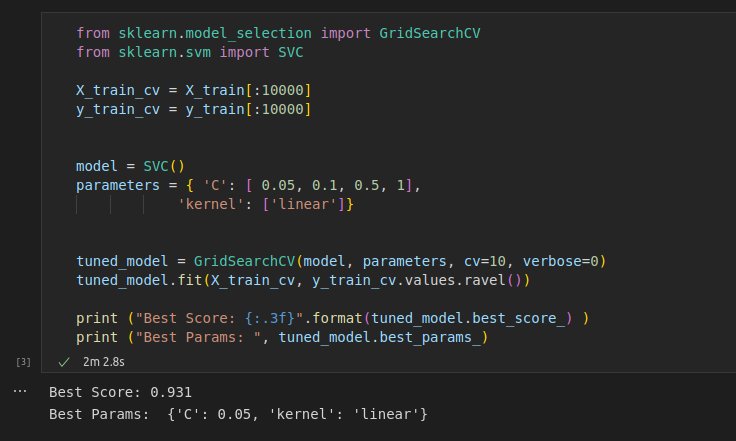
\includegraphics[scale=0.54]{linear_cross.png}
    \caption{Linear kernel cross validation}
    \label{fig:linear_cross}
\end{figure}

After that we can proceed with the training and test of the classifier 
(Listing \ref{lst:svm_linear}).

\begin{python}[caption={SVM linear kernel},label={lst:svm_linear}]
from sklearn import svm

#Create a svm Classifier with linear kernel
clf = svm.SVC(C=0.05,kernel='linear') # 

#Train the model using the training sets
clf.fit(X_train, y_train)

#Predict the response for test dataset
y_pred = clf.predict(X_test)
\end{python}
    

\subsubsection{Polynomial kernel}

The cross validation for the polynomial kernel classifier reveals (Figure \ref{fig:poly_cross}) that the best 
value of the parameter C is 5.

\begin{figure}[H]
    \centering
    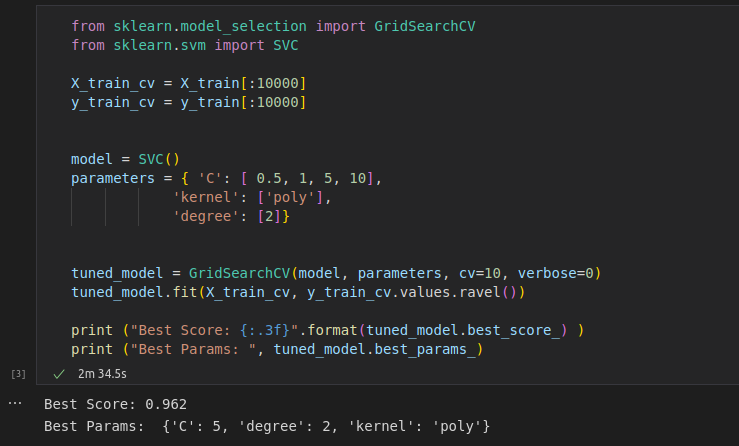
\includegraphics[scale=0.54]{poly_cross.png}
    \caption{Polynomial kernel cross validation}
    \label{fig:poly_cross}
\end{figure}

After that we can proceed with the training and test of the classifier 
(Listing \ref{lst:poly_linear}).

\begin{python}[caption={SVM polynomial kernel},label={lst:poly_linear}]
from sklearn import svm

#Create a svm Classifier with polynomial kernel
clf = svm.SVC(C=5,kernel='poly', degree=2)  # degree 2

#Train the model using the training sets
clf.fit(X_train, y_train)

#Predict the response for test dataset
y_pred = clf.predict(X_test)
\end{python}

\subsubsection{Radial Basis Function}
The cross validation for the RBF kernel classifier reveals (Figure \ref{fig:rbf_cross}) that the best 
value of the parameter C is 50.

\begin{figure}[H]
    \centering
    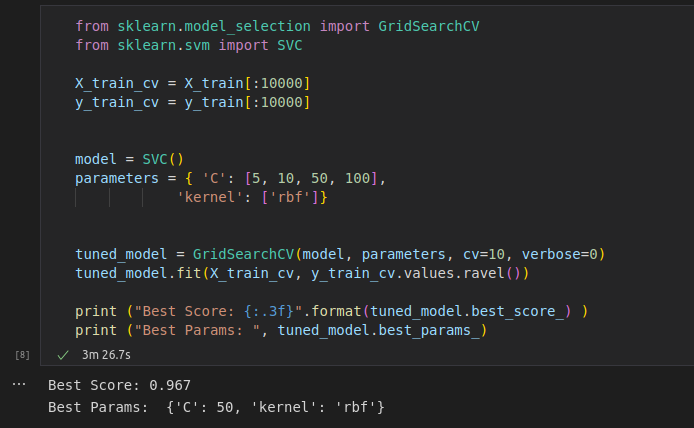
\includegraphics[scale=0.54]{rbf_cross.png}
    \caption{RBF kernel cross validation}
    \label{fig:rbf_cross}
\end{figure}

After that we can proceed with the training and test of the classifier 
(Listing \ref{lst:poly_linear}).

\begin{python}[caption={SVM RBF kernel},label={lst:rbf_linear}]
from sklearn import svm

#Create a svm Classifier RBF kernel
clf = svm.SVC(C=50,kernel='rbf') 

#Train the model using the training sets
clf.fit(X_train, y_train)

#Predict the response for test dataset
y_pred = clf.predict(X_test)
\end{python}


\subsection{Random forests}
For Random forests I used the \textbf{sklearn} library that implements the random 
forests classifier.
The cross validation is used to perform the tuning of the number of trees in the 
forest and it reveals (Figure \ref{fig:rf_cross}) that the optimum number of trees in the forest is 500.

\begin{figure}[H]
    \centering
    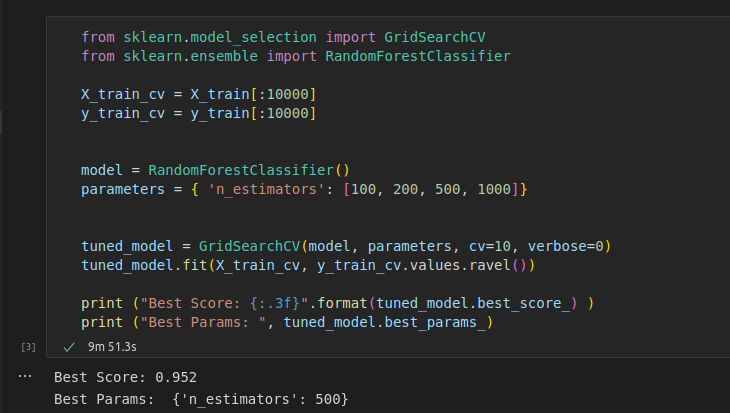
\includegraphics[scale=0.54]{rf_cross.png}
    \caption{RBF kernel cross validation}
    \label{fig:rf_cross}
\end{figure}

So we can proceed with the training and test of the classifier 
(Listing \ref{lst:random_forests}).

\begin{python}[caption={Random forests},label={lst:random_forests}]
from sklearn import svm

#Create a random forests Classifier
clf=RandomForestClassifier(n_estimators=500)

#Train the model using the training sets
clf.fit(X_train, y_train)

#Predict the response for test dataset
y_pred = clf.predict(X_test)
\end{python}

\subsection{Naive Bayes classifier}

For the Naive Bayes classifier we have to implement it by ourself.

The \verb|fit(self, X_train, y_train)| method(Listing \ref{lst:fit_naive}) creates 
the models for every class of the
training set ($[0 \dots 9]$) using the beta distribution; it's calculate the means
and the variances of the features of the data on the training set. After that it
calculates all the parameters needed to define the beta distribution, that models the 
class, and to calculates the joint pribabilities.

\begin{python}[caption={Naive Bayes fit method},label={lst:fit_naive}]
def fit(self, X_train, y_train):
    self.X_train = X_train
    self.y_train = y_train
    self.alphas = [None] * 10
    self.betas = [None] * 10
    self.p_class = [None] * 10

    for c in range(10):
        x_class_n = self.X_train[self.y_train == c]

        means = np.mean(x_class_n, axis=0)
        variances = np.var(x_class_n, axis=0)            
        
        ks = ((means * (1 - means)) / variances) - 1
        alphas = ks * means
        betas = ks * (1 - means)

        n_y_class_c = len(self.y_train[self.y_train == c])

        p_class = n_y_class_c / len(self.y_train)

        self.alphas[c] = np.array(alphas)
        self.betas[c] = np.array(betas)
        self.p_class[c] = np.array(p_class)
\end{python}

The \verb|predict(self, X)| method (Listing \ref{lst:predict_naive}) retrives
the parameters computed by the \verb|fit| method for every single class and then in 
order to calculate the joint distributions it calculates the $p(x_i|y=c)$ 
probabilities using the beta distribution. 

Since the beta distribution is a continuous
distribution is not possible to calculate $p(x_i|y=c)$, so I decided to calculate
the probability on a small neighbourhood of $x_i$, $p( x_i-0.05<x_i<x_i+0.05 | y=c)$ 
(I've choosen the value 0.05 after some tests). 
The computation of the beta probabilities in some cases can produce NaN as result, 
in this cases I've simply replaced the NaN values with 1 so that in the computation
of the joint distribution they are ignored.

After having calculated the joint probabilities for every single class, the 
\verb|predict| method selects the class with the higher joint probability.

\pagebreak
\begin{python}[caption={Naive Bayes fit method},label={lst:predict_naive}]
def predict(self, X):

    predict = np.array([])

    for index, row in X.iterrows():

        p = 0
        _class = None
        row = np.array(row)

        for c in range(10):

            alphas = self.alphas[c]
            betas = self.betas[c]
            p_class = self.p_class[c]
            
            betas_plus = beta.cdf(row+0.05, alphas, betas)
            betas_minus = beta.cdf(row-0.05, alphas, betas)
            beta_probs = betas_plus - betas_minus
            
            np.nan_to_num(beta_probs, copy=False, nan=1.0)
            p_temp = np.product(beta_probs) * p_class
            

            if p_temp >= p:
                p = p_temp
                _class = c
        
        predict = np.append(predict, _class)
    
    return predict
\end{python}

On this Naive Bayes classifier there are no parameters to be tuned so we can simply
proceed with the training and test of the classifier (Label \ref{lst:naive_bayes}).
\pagebreak
\begin{python}[caption={Naive Bayes classifier},label={lst:naive_bayes}]
    #Create a Naive Bayes Classifier
    clf = beta_NaiveBayes() 

    #Train the model using the training sets
    clf.fit(X_train, y_train)
    
    #Predict the response for test dataset
    y_pred = clf.predict(X_test)
\end{python}

\subsection{k-nearest neighbors (k-NN)}

For the k-NN we have to implement it by ourself. 

First of all the \verb|fit(self, X_train, y_train)| (Listing \ref{lst:knn_fit}) 
is implemented simply
by saving the training set as numpy arrays.

\begin{python}[caption={k-NN fit method},label={lst:knn_fit}]
def fit(self, X_train, y_train):
    self.X_train = np.array(X_train)
    self.y_train = np.array(y_train)
\end{python}

Then let's define the method \verb|predict(self, X)| (Listing \ref{lst:knn_predict}) 
to classify new data; it simply iterates through every single point in input and 
with the help of the \verb|__supp| private method it finds the distance to every 
points on the training set and selects the classes of the k nearest points. 
After that with the \verb|statistics.mode| function it selects the most common 
class on the k selected.

\pagebreak
\begin{python}[caption={k-NN predict method},label={lst:knn_predict}]
def __supp(self, x):
    distances = np.linalg.norm(x - self.X_train, axis=1)
    neighbors_y = self.y_train[np.argsort(distances)[:self.k]]

    return statistics.mode(neighbors_y)


def predict(self, X):
    X = np.array(X)
    predict = np.array([])

    for x in X:
        predict = np.append(predict, self.__supp(x))

    return predict
\end{python}

The cross validation is used to perform the tuning of the number of neighbors to take
in condideration and it reveals (Figure \ref{fig:knn_cross}) that the optimum number of neighbors is 5.

\begin{figure}[H]
    \centering
    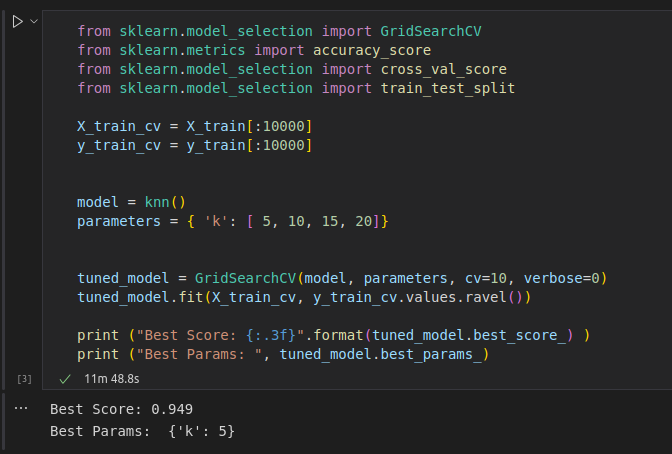
\includegraphics[scale=0.6]{knn_cross.png}
    \caption{k-NN cross validation}
    \label{fig:knn_cross}
\end{figure}

After having implemented the k-NN classifier we can proceed with the training and 
test of the classifier (Listing \ref{lst:knn}).

\begin{python}[caption={k-NN},label={lst:knn}]
#Create a k-NN Classifier
clf = knn(k=5) 

#Train the model using the training sets
clf.fit(X_train, y_train)

#Predict the response for test dataset
y_pred = clf.predict(X_test)
\end{python}

\section{Considerations}

In the table \ref{tbl:classifiers_comparison} is shown a comparison between all the 
classifier on this report.

As we can see all the SVM classifiers have similar computational (time) requirements
on cross validation, training and test time. The polynomial and RBF kernel 
classifiers seem to have an higher accuracy on the prediction on the training set with 
,as already said, similar computational requirements than the linear kernel 
classifier.

The random forests classifiers seems to have slightly less accuracy than the SVM
classifiers and a similar training time, the prediction time instead is way smaller
than the SVM ones. I've also made a test reducing to 200 the number of trees in the 
forest to see how the performance changes; as expected, because of the cross 
validation, the accuracy is smaller but by
a very small amount, 0.9681 for the 200 trees forests againt 0.9686 for the 500 
trees forest. However on the performance side the training time decreases significally
to 57 seconds, against the 2 minutes and 22 seconds of the 500 trees forest; so for 
this reason it may be convenient to use the classifier with the 200 trees forest. 

\begin{table}[H]
   \begin{center}
             \begin{tabular}{||c | c | c | c | c ||}
             \hline
             Classifier & Accuracy & CV time  & Training time & Test time  \\ [0.5ex]
             \hline
             SVM linear  & 0.9429 & 2m 2s & 2m 8s & 41s\\ [1ex]
             SVM poly  & 0.9802 & 2m 34s & 1m 52s & 31s\\ [1ex]
             SVM RBF  & 0.9820 & 3m 26s & 2m 22s & 54s\\ [1ex]
             Random forests  & 0.9686 & 9m 51s & 2m 20s & 1.3s\\ [1ex]
             Naive Bayes classifier  & 0.8399 & - & 0.4s & 43s\\ [1ex]
             k-NN  & 0.9719 & 11m 49s & 0.8s & 27m 12s\\ [1ex]
             \hline
             \end{tabular}
             \caption{Classifiers comparison}
             \label{tbl:classifiers_comparison}
   \end{center}
\end{table}
   


\end{document}